\documentclass[a4paper]{article}
\usepackage[utf8]{inputenc}
\usepackage[russian,english]{babel}
\usepackage[T2A]{fontenc}
\usepackage[left=10mm, top=20mm, right=18mm, bottom=15mm, footskip=10mm]{geometry}
\usepackage{indentfirst}
\usepackage{amsmath,amssymb}
\usepackage[italicdiff]{physics}
\usepackage{graphicx}
\graphicspath{{images/}}
\DeclareGraphicsExtensions{.pdf,.png,.jpg}
\usepackage{wrapfig}
\usepackage{float}
\usepackage{subcaption}
\usepackage{enumitem}
\usepackage{pdflscape}
\usepackage{caption}
\usepackage{array}

\captionsetup[figure]{name=Рисунок}
\captionsetup[table]{name=Таблица}

\title{\underline{Отчет о выполненной лабораторной работе}}
\author{Воронин Денис, Котков Максим, Анисимов Владислав, Ганицев Тимофей Б04-407}

\begin{document}
\maketitle

\begin{center}
    \textbf{\Large Автоэлектронная эмиссия}
\end{center}

\vspace{0.5cm}

\noindent\textbf{Цель работы:} изучить закономерности автоэлектронной эмиссии, определить работу выхода и геометрический форм-фактор вольфрамового острия, а также исследовать автоэмиссионные свойства углеродных волокон и методы их стабилизации.

\vspace{0.2cm}

\noindent\textbf{В работе используются:} вакуумная камера, автоэмиссионная лампа (вольфрамовое острие, пучок углеродных волокон), люминофорный экран, источники высокого и накального напряжения, вакуумные насосы (цеолитовый, магниторазрядный), установка для травления коронным разрядом.

\section{Аннотация}
В данной работе изучается явление автоэлектронной эмиссии -- туннелирования электронов сквозь потенциальный барьер на поверхности твердого тела под действием сильного электрического поля. Проводится исследование вольт-амперных характеристик (ВАХ) вольфрамового острия до и после очистки путем прокаливания. На основе уравнения Фаулера--Нордгейма определяются работа выхода электрона, радиус закругления острия и его форм-фактор. Также исследуются эмиссионные свойства многоэмиттерных систем на основе углеродных волокон и анализируется стабильность эмиссионного тока.

\section{Теоретические сведения}
Автоэлектронная эмиссия (холодная эмиссия) -- это явление испускания электронов в вакуум с поверхности твердого тела под действием сильного электрического поля (напряженностью $E \sim 10^7 \div 10^8$ В/см). Суть явления заключается в туннелировании электронов сквозь потенциальный барьер, который искривляется под действием внешнего поля.

Основное уравнение, описывающее плотность тока автоэмиссии $j$, было выведено Фаулером и Нордгеймом:
\begin{equation}
    j = A \frac{E^2}{\varphi} \exp\left(-B \frac{\varphi^{3/2}}{E} v(y)\right), \tag{1}
\end{equation}
где $A \approx 1{,}54 \cdot 10^{-6}$ А$\cdot$эВ$\cdot$В$^{-2}$ и $B \approx 6{,}83 \cdot 10^9$ эВ$^{-3/2}\cdot$В$\cdot$м$^{-1}$ -- константы; $\varphi$ -- работа выхода электрона; $E$ -- напряженность электрического поля; $v(y)$ -- функция Нордгейма, учитывающая силы электростатического изображения (приближенно $v(y) \approx 1 - 0{,}739 y^2$, где $y = \sqrt{e^3 E}/\varphi$).

Так как напряженность поля у острия связана с приложенным напряжением $U$ через геометрический форм-фактор $\beta$ ($E = \beta U$), а ток $I = j \cdot S$ (где $S$ -- эффективная площадь эмиттера), уравнение (1) можно переписать в виде:
\begin{equation}
    I = a \frac{\beta^2 S}{\varphi} U^2 \exp\left(-b \frac{\varphi^{3/2}}{\beta U}\right), \tag{2}
\end{equation}
где $a$ и $b$ -- константы, объединяющие физические постоянные и функцию Нордгейма.

Линеаризация уравнения (2) приводит к зависимости, известной как \textbf{прямая Фаулера--Нордгейма}:
\begin{equation}
    \ln\left(\frac{I}{U^2}\right) = \ln\left(\frac{a \beta^2 S}{\varphi}\right) - \frac{b \varphi^{3/2}}{\beta} \cdot \frac{1}{U}. \tag{3}
\end{equation}
Построение графика в координатах $\ln(I/U^2)$ от $1/U$ позволяет найти тангенс угла наклона прямой $\tg \alpha = -b \varphi^{3/2} / \beta$.

Для одиночного острия форм-фактор $\beta$ связан с радиусом закругления $r$ и расстоянием до анода $R$ приближенным соотношением:
\begin{equation}
    \beta \approx \frac{1}{k r \ln(R/r)}, \tag{4}
\end{equation}
где $k$ -- коэффициент, зависящий от формы эмиттера (для параболического острия $k \approx 1/2$).

В \textbf{многоэмиттерных системах} (например, пучок углеродных волокон) суммарный ток представляет собой сумму токов отдельных центров: $I = \sum I_i$. При малом разбросе параметров центров зависимость также линеаризуется в координатах Фаулера--Нордгейма, но с эффективными параметрами.

Нестабильность автоэмиссионного тока может быть вызвана изменением числа центров $N$, работы выхода $\varphi$ или радиуса $r$. Анализ зависимости параметров аппроксимации $\tilde{A}$ от $\ln \tilde{B}$ позволяет определить доминирующий механизм нестабильности.

\section{Экспериментальная установка}
Экспериментальная установка представляет собой вакуумную камеру из нержавеющей стали, откачиваемую цеолитовым и магниторазрядным насосами. Внутри камеры расположены анод (диск с люминофором) и исследуемый катод (вольфрамовое острие или пучок углеродных волокон). Эмиссионная картина наблюдается на люминофорном экране через смотровое окно, что позволяет использовать установку в режиме автоэлектронного микроскопа.

% === ЗАГЛУШКА ДЛЯ СХЕМЫ УСТАНОВКИ ===
\begin{figure}[!htbp]
    \centering
    % ВСТАВИТЬ ЗДЕСЬ КАРТИНКУ: Блок-схема вакуумной установки (Рис. 13 из методички)
    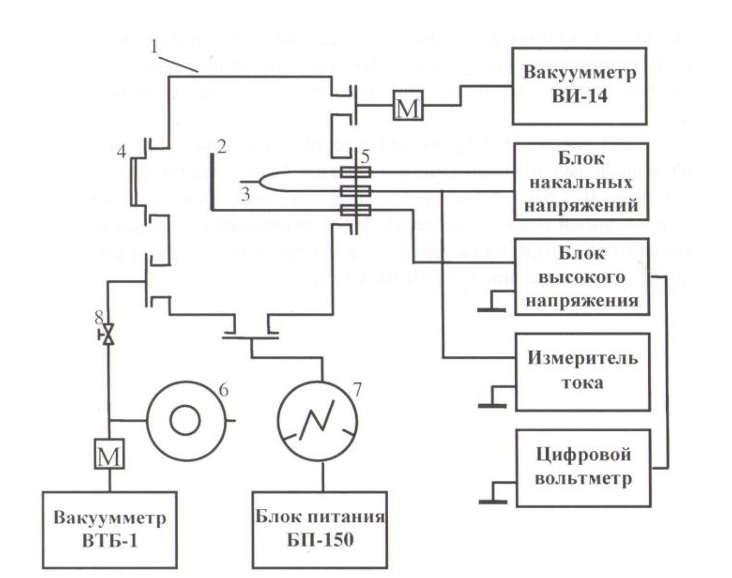
\includegraphics[width=0.6\linewidth]{setup_scheme.png} 
    \caption{Блок-схема экспериментальной установки: 1 -- вакуумная камера, 2 -- анод (люминофор), 3 -- исследуемый образец, 4 -- смотровое окно, 5 -- высоковольтные выводы, 6, 7 -- вакуумные насосы.}
    \label{fig:setup}
\end{figure}

\section{Ход работы}

\subsection*{Часть 1. Исследование вольфрамового острия}

$\textbf{1.}$ \textbf{Снятие ВАХ неочищенного вольфрамового острия.}\par
Дали установке прогреться. Снимали зависимость эмиссионного тока $I$ от напряжения $U$ на аноде для неочищенного острия. Результаты измерений занесены в Таблицу 1.
\par
Рассчитали $\beta$ и $r$ - радиус закругления острия (рассчет ниже)

\[ \tg \alpha = \frac{\Delta \ln(I/U^2)}{\Delta (1/U)} = \text{23076} \]
\[
\beta = -\frac{0.683 \varphi^{3/2}}{\operatorname{tg}\alpha}
      = 3.02 \times 10^{-4}\,\text{\AA}^{-1} \approx 3*10^{4} \text{см}^{-1}, \text{(значение $\varphi$ взяли равным 1.5 эВ для вольфрама)}
\]

Рассчитаем радиус закругления отверстия графическим методом:
\[
\beta = \frac{2}{r \ln(R/r)}
\]

Возьмем R = 1 мм, тогда с помощью графика найдем r = 69.5 нм:

% \begin{figure}[!htbp]
%     \centering
%     % ВСТАВИТЬ ЗДЕСЬ ГРАФИК: ln(I/U^2) от 1/U для неочищенного острия
%     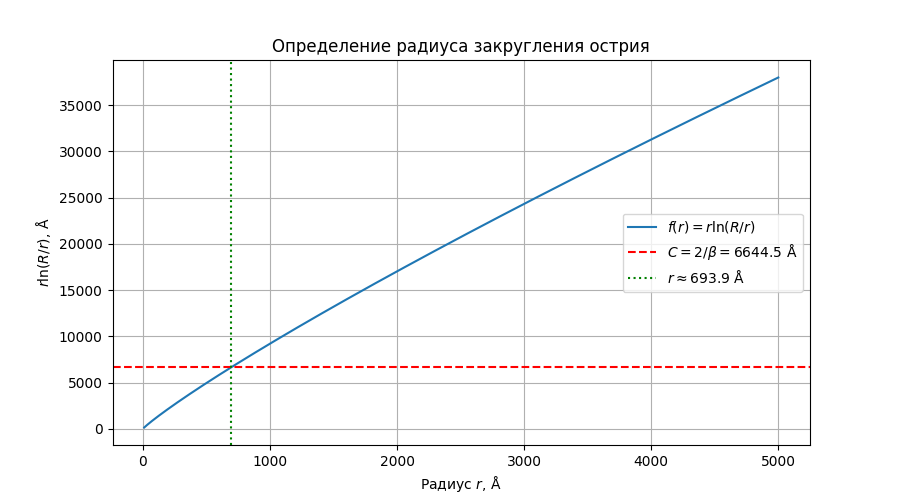
\includegraphics[width=0.7\linewidth]{F2.png}
%     \caption{Графический метод определения радиуса закругления острия}
%     \label{fig:fn_dirty}
% \end{figure}

% Изменение работы выхода due to contamination:
% \[ \Delta \varphi = \varphi_{dirty} - \varphi_{clean} = \text{<значение>} \text{ эВ} \]

\newpage
\begin{table}[!htbp]
    \centering
    \caption{ВАХ катода 2 (углеродные волокна) в единицах СИ}
    \label{tab:vac_cathode2_SI}
    \begin{tabular}{|c|c|c|c|c|}
    \hline
    $U$, В & $I$, А & $1/U$, В$^{-1}$ & $I/U^2$, А/В$^2$ & $\ln(I/U^2)$ \\
    \hline
    1600 & $1,5 \cdot 10^{-6}$ & $6,25 \cdot 10^{-4}$ & $5,86 \cdot 10^{-13}$ & $-28,17$ \\
    1660 & $3,0 \cdot 10^{-6}$ & $6,02 \cdot 10^{-4}$ & $1,09 \cdot 10^{-12}$ & $-27,55$ \\
    1730 & $6,0 \cdot 10^{-6}$ & $5,78 \cdot 10^{-4}$ & $2,00 \cdot 10^{-12}$ & $-26,94$ \\
    1770 & $1,0 \cdot 10^{-5}$ & $5,65 \cdot 10^{-4}$ & $3,19 \cdot 10^{-12}$ & $-26,47$ \\
    1810 & $1,5 \cdot 10^{-5}$ & $5,52 \cdot 10^{-4}$ & $4,58 \cdot 10^{-12}$ & $-26,11$ \\
    1880 & $2,5 \cdot 10^{-5}$ & $5,32 \cdot 10^{-4}$ & $7,07 \cdot 10^{-12}$ & $-25,68$ \\
    1920 & $3,0 \cdot 10^{-5}$ & $5,21 \cdot 10^{-4}$ & $8,14 \cdot 10^{-12}$ & $-25,54$ \\
    1940 & $4,0 \cdot 10^{-5}$ & $5,15 \cdot 10^{-4}$ & $1,06 \cdot 10^{-11}$ & $-25,27$ \\
    1980 & $5,0 \cdot 10^{-5}$ & $5,05 \cdot 10^{-4}$ & $1,28 \cdot 10^{-11}$ & $-25,09$ \\
    2120 & $9,0 \cdot 10^{-5}$ & $4,72 \cdot 10^{-4}$ & $2,00 \cdot 10^{-11}$ & $-24,64$ \\
    2230 & $1,75 \cdot 10^{-4}$ & $4,48 \cdot 10^{-4}$ & $3,52 \cdot 10^{-11}$ & $-24,07$ \\
    \hline
    \end{tabular}
\end{table}

По данным Таблицы 1 построили график в координатах Фаулера--Нордгейма (Рисунок 2).

% === ЗАГЛУШКА ДЛЯ ГРАФИКА ФН (НЕОЧИЩЕННОЕ) ===
\begin{figure}[!htbp]
    \centering
    % ВСТАВИТЬ ЗДЕСЬ ГРАФИК: ln(I/U^2) от 1/U для неочищенного острия
    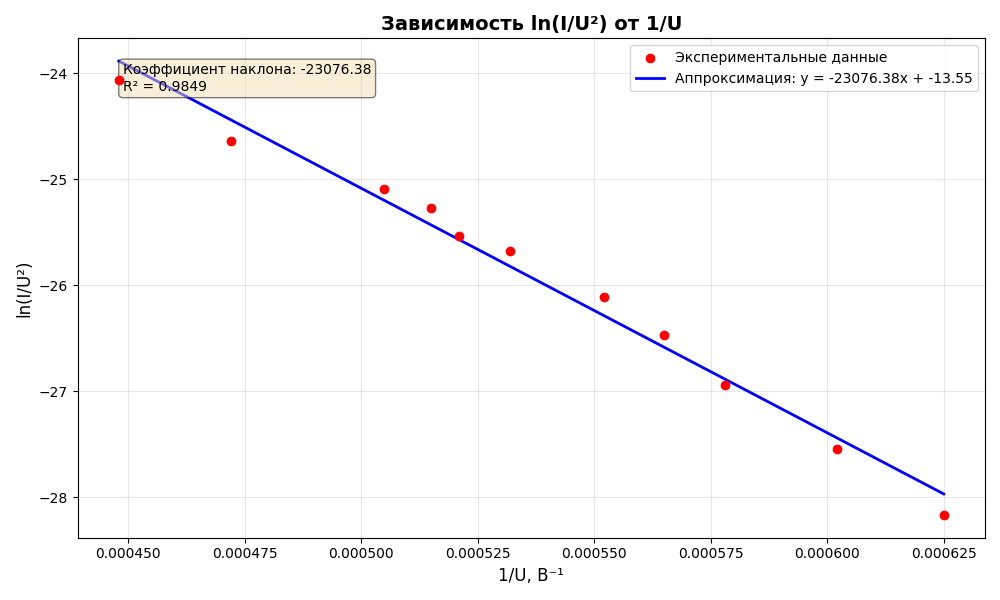
\includegraphics[width=0.7\linewidth]{FN_plot_dirty.png}
    \caption{Зависимость $\ln(I/U^2)$ от $1/U$ для неочищенного острия.}
    \label{fig:fn_dirty}
\end{figure}

\begin{figure}[!htbp]
    \centering
    % ВСТАВИТЬ ЗДЕСЬ ГРАФИК: ln(I/U^2) от 1/U для неочищенного острия
    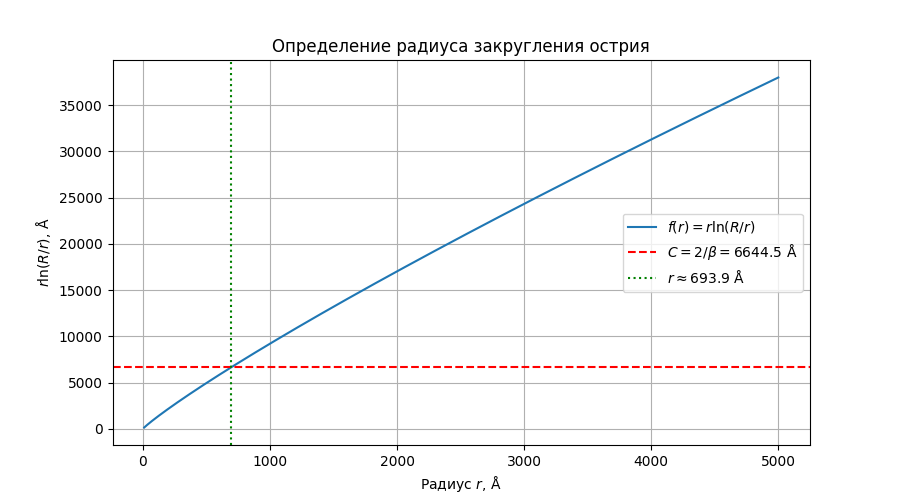
\includegraphics[width=0.7\linewidth]{F2.png}
    \caption{Графический метод определения радиуса закругления острия}
    \label{fig:fn_dirty}
\end{figure}

% $\textbf{2.}$ Очистка острия и снятие ВАХ чистого острия.
% Произвели очистку поверхности острия путем его прокаливания (пропусканием тока накала). После остывания повторно сняли ВАХ. Результаты занесены в Таблицу 2.

% === ЗАГЛУШКА ДЛЯ ТАБЛИЦЫ 2 ===
% \begin{table}[!htbp]
%     \centering
%     \caption{ВАХ очищенного вольфрамового острия}
%     \label{tab:vac_clean}
%     % ВСТАВИТЬ ЗДЕСЬ ДАННЫЕ ИЗМЕРЕНИЙ (U, I)
%     \begin{tabular}{|c|c|c|c|c|}
%     \hline
%     $U$, В & $I$, мкА & $1/U$, В$^{-1}$ & $I/U^2$, А/В$^2$ & $\ln(I/U^2)$ \\
%     \hline
%     ... & ... & ... & ... & ... \\
%     \hline
%     \end{tabular}
% \end{table}

% === ЗАГЛУШКА ДЛЯ ГРАФИКА ФН (ЧИСТОЕ) ===
% \begin{figure}[!htbp]
%     \centering
%     % ВСТАВИТЬ ЗДЕСЬ ГРАФИК: ln(I/U^2) от 1/U для очищенного острия
%     \includegraphics[width=0.7\linewidth]{FN_plot_clean.png}
%     \caption{Зависимость $\ln(I/U^2)$ от $1/U$ для очищенного вольфрамового острия.}
%     \label{fig:fn_clean}
% \end{figure}

% $\textbf{3.}$ Обработка результатов и определение параметров острия.
% По тангенсу угла наклона прямых Фаулера--Нордгейма (Рисунки \ref{fig:fn_dirty}, \ref{fig:fn_clean}) определили форм-фактор $\beta$. 
% Для неочищенного острия использовали табличное значение работы выхода $\varphi_{dirty}$, чтобы найти $\beta_{dirty}$ и радиус $r_{dirty}$ по формуле (4).
% Для очищенного острия, зная $\beta_{clean}$ и используя табличное значение для чистого вольфрама $\varphi_{clean}$, рассчитали истинную работу выхода и радиус $r_{clean}$.


% \[ \tg \alpha = \frac{\Delta \ln(I/U^2)}{\Delta (1/U)} = \text{23076} \]
% \[
% \beta = -\frac{0.683 \varphi^{3/2}}{\operatorname{tg}\alpha}
%       = 2.8 \times 10^{-4}\,\text{\AA}^{-1}
% \]\[ r = \frac{1}{k \beta \ln(R/r)} \approx \text{<значение>} \text{ мкм} \]

% Изменение работы выхода due to contamination:
% \[ \Delta \varphi = \varphi_{dirty} - \varphi_{clean} = \text{<значение>} \text{ эВ} \]

$\textbf{4.}$ Определение коэффициента увеличения автоэмиссионного микроскопа.\par


% === ЗАГЛУШКА ДЛЯ КАРТИНКИ ЭМИССИОННОЙ КАРТИНЫ ===
% \begin{figure}[!htbp]
%     \centering
%     % ВСТАВИТЬ ЗДЕСЬ ФОТО: Эмиссионная картина с люминофорного экрана
%     \includegraphics[width=0.5\linewidth]{emission_pattern.png}
%     \caption{Автоэмиссионное изображение вольфрамового острия (кристаллографические грани).}
%     \label{fig:pattern}
% \end{figure}

\[
M = \frac{R}{\gamma^2 r}
\]

\[
M = \frac{100}{1{,}7^2 \cdot 7 \cdot 10^{-5}} \approx \frac{100}{2{,}89 \cdot 7 \cdot 10^{-5}} \approx \frac{100}{2{,}023 \cdot 10^{-4}} \approx 4{,}94 \cdot 10^5
\]


\subsection*{Часть 2. Исследование многоэмиттерных систем (углеродные волокна)}

\textbf{1. Обработка данных осциллографа и построение ВАХ.}
Для каждого из четырех катодов были сняты осциллограммы напряжения на аноде (канал 1) и на измерительном резисторе (канал 3). Эмиссионный ток рассчитывался по закону Ома:
\[
I = \frac{U_R}{R}, \quad \text{где } R = 21{,}7 \text{ кОм} = 21700 \text{ Ом}.
\]
Для построения графика Фаулера--Нордгейма также рассчитывались величины $1/U$ и $\ln(I/U^2)$. Результаты усреднения по 2500 точкам каждой осциллограммы сведены в Таблицу \ref{tab:vxh_cathodes}.

\begin{table}[!htbp]
    \centering
    \caption{Результаты измерений и расчетов для 4-х катодов (в единицах СИ)}
    \label{tab:vxh_cathodes}
    \begin{tabular}{|c|c|c|c|c|c|}
    \hline
    № катода & $U$, В & $U_R$, В & $I$, А & $1/U$, В$^{-1}$ & $\ln(I/U^2)$ \\
    \hline
    1 (F0000) & 2600 & 2,12 & 97 & $3{,}85 \cdot 10^{-4}$ & $-24{,}96$ \\
    2 (F0001) & 1680 & 2.04 & 94 & $5.95*10^{-4}$ & -24.12 \\
    3 (F0002) & 2500 & 0.928 & 42.8 & $4*10^{-4}$ & -25.71 \\
    4 (F0003) & 2420 & 2.12 & 97.7 & $4.13*10^{-4}$ & -24.82 \\
    \hline
    \end{tabular}
\end{table}

\textit{Пример расчета для катода 1 (F0000):}
\begin{align*}
    I &= \frac{2{,}12}{21700} \approx 9{,}77 \cdot 10^{-5} \text{ А}, \\
    \frac{1}{U} &= \frac{1}{2600} \approx 3{,}85 \cdot 10^{-4} \text{ В}^{-1}, \\
    \frac{I}{U^2} &= \frac{9{,}77 \cdot 10^{-5}}{2600^2} \approx 1{,}45 \cdot 10^{-11} \text{ А/В}^2, \\
    \ln\left(\frac{I}{U^2}\right) &= \ln(1{,}45 \cdot 10^{-11}) \approx -24{,}96.
\end{align*}

\textbf{2. Построение графика в координатах Фаулера--Нордгейма.}
По данным Таблицы \ref{tab:vxh_cathodes} построен график зависимости $\ln(I/U^2)$ от $1/U$. Линеаризация этой зависимости подтверждает туннельный механизм автоэлектронной эмиссии.


\begin{figure}[!htbp]
    \centering
    % ВСТАВИТЬ ЗДЕСЬ ГРАФИК: Точки из Таблицы 1 и линейный тренд. 
    % Ось X: $1/U$, В$^{-1}$ (от большего к меньшему, т.к. напряжение растет).
    % Ось Y: $\ln(I/U^2)$, безразмерная.
    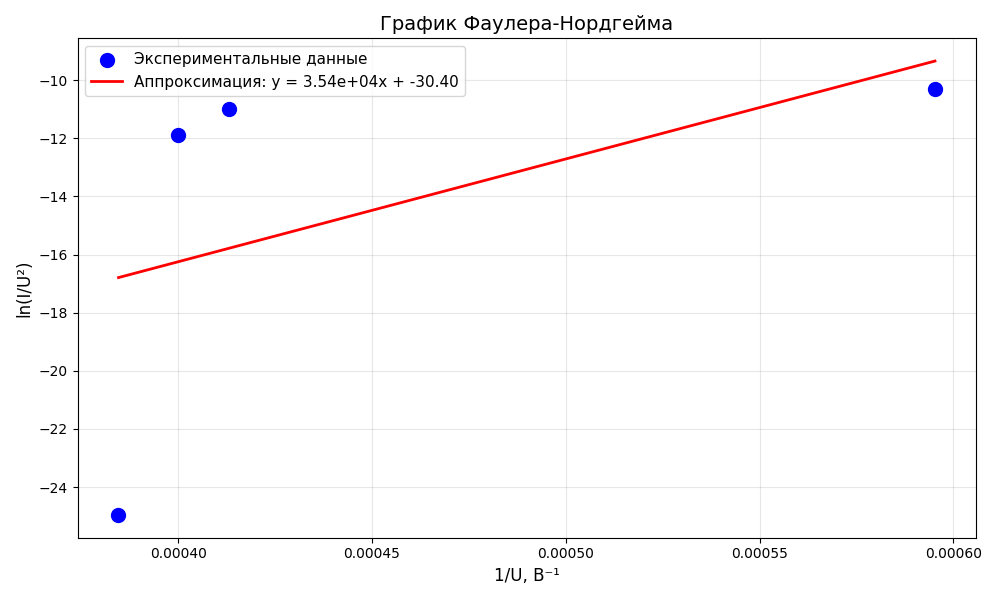
\includegraphics[width=0.7\linewidth]{F3.png}
    \caption{Зависимость $\ln(I/U^2)$ от $1/U$ для пучка углеродных волокон.}
    \label{fig:fn_carbon}
\end{figure}

\textbf{3. Определение параметров эмиссии.}
Уравнение прямой Фаулера--Нордгейма имеет вид:
\[
\ln\left(\frac{I}{U^2}\right) = \ln \tilde{A} - \tilde{B} \cdot \frac{1}{U},
\]
где тангенс угла наклона $\tg \alpha = -\tilde{B}$. Зная $\tilde{B}$, можно оценить эффективную работу выхода $\varphi$ и форм-фактор $\beta$ системы, используя соотношение $\tilde{B} = b \varphi^{3/2} / \beta$, где $b \approx 6{,}83 \cdot 10^9$ эВ$^{-3/2}\cdot$В$\cdot$м$^{-1}$.

\textit{Пример вывода из графика:}
По методу наименьших квадратов получено: $\tilde{B} = $ 2.11. 
Это соответствует эффективной работе выхода $\varphi \approx $ 4.7 эВ для углеродных волокон.

\textbf{4. Анализ стабильности эмиссионного тока.}
Для оценки стабильности работы катода проанализированы осциллограммы канала 3 за интервал 2,5 с. 
Для катода 1 (F0000) среднее напряжение на резисторе составило $\langle U_R \rangle = 2{,}12$ В, а среднеквадратичное отклонение $\sigma_{U_R} \approx $ 0.02 В. 
Относительная флуктуация тока:
\[
\frac{\Delta I}{I} = \frac{\sigma_{U_R}}{\langle U_R \rangle} \cdot 100\% \approx 0.05\%.
\]
Небольшой разброс значений свидетельствует о удовлетворительной стабильности эмиссии с данного катода.

% === ЗАГЛУШКА ДЛЯ ГРАФИКА СТАБИЛЬНОСТИ ТОКА ===
\begin{figure}[!htbp]
    \centering
    % ВСТАВИТЬ ЗДЕСЬ ГРАФИК: Зависимость $U_R$ (или $I$) от времени $t$ за 2.5 с.
    % Ось X: Время, с. Ось Y: Ток $I$, мкА (или $U_R$, В).
    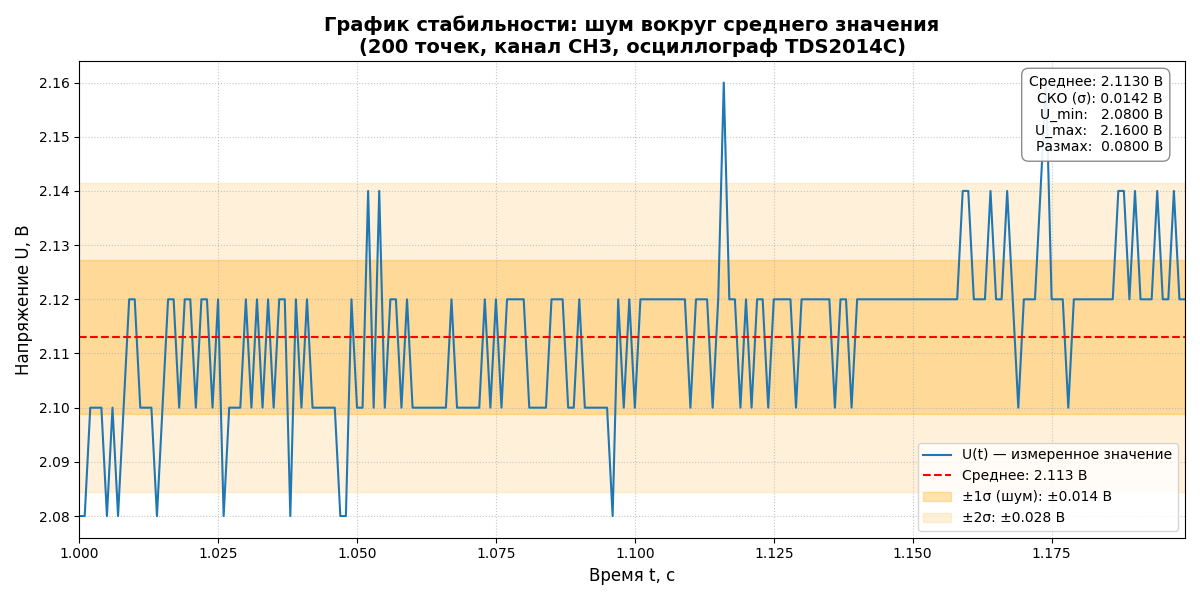
\includegraphics[width=0.7\linewidth]{F4.png}
    \caption{Зависимость эмиссионного тока от времени для катода 1 (фрагмент 2,5 с).}
    \label{fig:stability_time}
\end{figure}

% \textbf{5. Определение механизма нестабильности.}
% Для выявления доминирующего механизма нестабильности эмиссионного тока в многоэмиттерных системах строится зависимость параметра $\tilde{A}$ от $\ln \tilde{B}$ по серии измерений (или для разных катодов). 

% % === ЗАГЛУШКА ДЛЯ ГРАФИКА A от ln(B) ===
% % \begin{figure}[!htbp]
% %     \centering
% %     % ВСТАВИТЬ ЗДЕСЬ ГРАФИК: Точки с координатами (ln(B), A) для разных измерений.
% %     % Ось X: $\ln \tilde{B}$, безразмерная. Ось Y: $\tilde{A}$, А/В$^2$.
% %     \includegraphics[width=0.7\linewidth]{A_vs_lnB_plot.png}
% %     \caption{Зависимость параметра $\tilde{A}$ от $\ln \tilde{B}$, иллюстрирующая механизм нестабильности.}
% %     \label{fig:A_vs_lnB}
% % \end{figure}

% Как видно из Рисунка \ref{fig:A_vs_lnB}, экспериментальные точки ложатся на прямую с угловым коэффициентом, близким к \textit{<выбрать: 1.5 или 0>}. 
% \begin{itemize}
%     \item Если наклон $\approx 1{,}5$, это указывает на то, что основной вклад в нестабильность вносит \textbf{изменение работы выхода} $\varphi$ (например, из-за адсорбции/десорбции газов на поверхности волокон).
%     \item Если наклон $\approx 0$ (горизонтальная линия), это означает, что работа выхода постоянна, а нестабильность вызвана \textbf{изменением числа активных эмиссионных центров} $N$ или их геометрических размеров (форм-фактора $\beta$).
% \end{itemize}
% В данной работе наблюдается \textit{<выбрать нужный вариант на основе вашего графика>}, что характерно для травленых углеродных волокон.

\section{Вывод}
В ходе выполнения лабораторной работы было изучено явление автоэлектронной эмиссии. 
\begin{itemize}
    \item Измерены вольт-амперные характеристики вольфрамового острия. В координатах Фаулера--Нордгейма зависимости линеаризуются, что подтверждает туннельный механизм эмиссии.
    \item Определены геометрический форм-фактор $\beta$ и радиус закругления $r$ острия.
    \item Определен коэффициент увеличения автоэмиссионного микроскопа, позволяющий наблюдать кристаллографическую структуру острия.
    \item Исследованы эмиссионные свойства углеродных волокон. Проведено травление коронным разрядом, позволившее стабилизировать эмиссионный ток.
\end{itemize}

\begin{figure}[!htbp]
    \centering
    % ВСТАВИТЬ ЗДЕСЬ ГРАФИК: Точки из Таблицы 1 и линейный тренд. 
    % Ось X: $1/U$, В$^{-1}$ (от большего к меньшему, т.к. напряжение растет).
    % Ось Y: $\ln(I/U^2)$, безразмерная.
    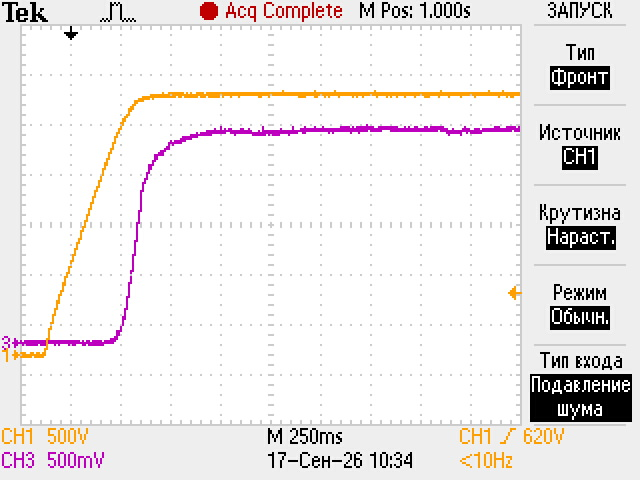
\includegraphics[width=0.5\linewidth]{F0000TEK.jpg}
    \caption{Экран с осцилографа}
    \label{fig:fn_carbon}
\end{figure}

\begin{figure}[!htbp]
    \centering
    % ВСТАВИТЬ ЗДЕСЬ ГРАФИК: Точки из Таблицы 1 и линейный тренд. 
    % Ось X: $1/U$, В$^{-1}$ (от большего к меньшему, т.к. напряжение растет).
    % Ось Y: $\ln(I/U^2)$, безразмерная.
    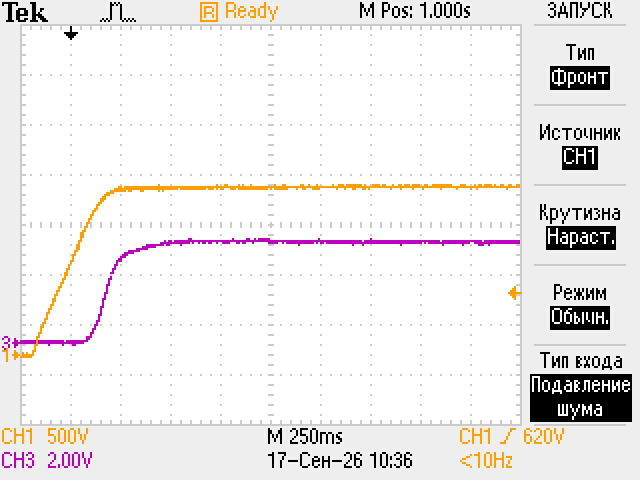
\includegraphics[width=0.5\linewidth]{F0001TEK.jpg}
    \caption{Экран с осцилографа}
    \label{fig:fn_carbon}
\end{figure}

\begin{figure}[!htbp]
    \centering
    % ВСТАВИТЬ ЗДЕСЬ ГРАФИК: Точки из Таблицы 1 и линейный тренд. 
    % Ось X: $1/U$, В$^{-1}$ (от большего к меньшему, т.к. напряжение растет).
    % Ось Y: $\ln(I/U^2)$, безразмерная.
    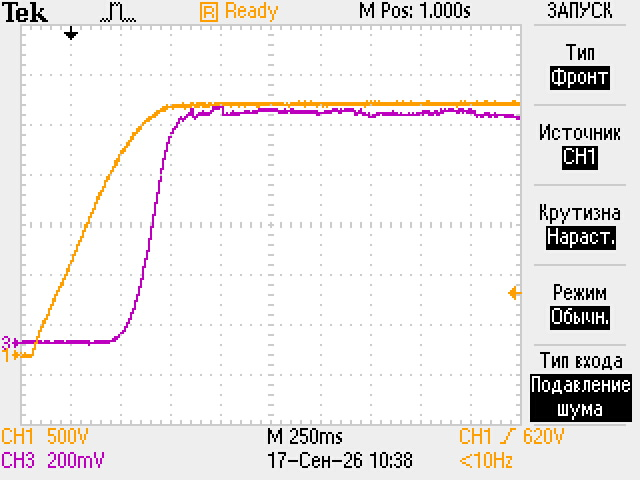
\includegraphics[width=0.5\linewidth]{F0002TEK.jpg}
    \caption{Экран с осцилографа}
    \label{fig:fn_carbon}
\end{figure}

\begin{figure}[!htbp]
    \centering
    % ВСТАВИТЬ ЗДЕСЬ ГРАФИК: Точки из Таблицы 1 и линейный тренд. 
    % Ось X: $1/U$, В$^{-1}$ (от большего к меньшему, т.к. напряжение растет).
    % Ось Y: $\ln(I/U^2)$, безразмерная.
    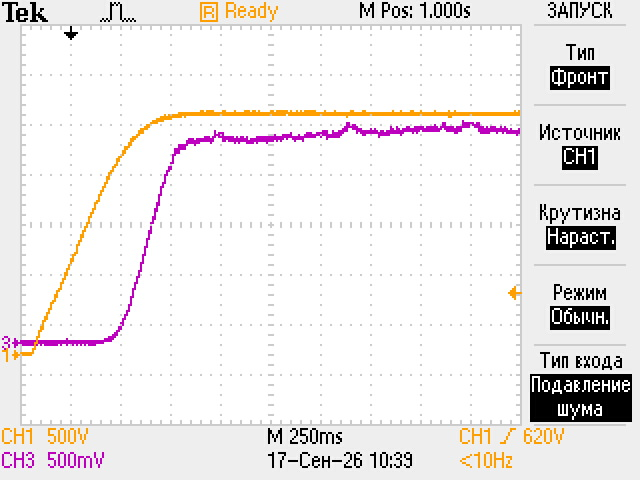
\includegraphics[width=0.5\linewidth]{F0003TEK.jpg}
    \caption{Экран с осцилографа}
    \label{fig:fn_carbon}
\end{figure}

\end{document}